% Options for packages loaded elsewhere
\PassOptionsToPackage{unicode}{hyperref}
\PassOptionsToPackage{hyphens}{url}
\documentclass[
]{article}
\usepackage{xcolor}
\usepackage{amsmath,amssymb}
\setcounter{secnumdepth}{-\maxdimen} % remove section numbering
\usepackage{iftex}
\ifPDFTeX
  \usepackage[T1]{fontenc}
  \usepackage[utf8]{inputenc}
  \usepackage{textcomp} % provide euro and other symbols
\else % if luatex or xetex
  \usepackage{unicode-math} % this also loads fontspec
  \defaultfontfeatures{Scale=MatchLowercase}
  \defaultfontfeatures[\rmfamily]{Ligatures=TeX,Scale=1}
\fi
\usepackage{lmodern}
\ifPDFTeX\else
  % xetex/luatex font selection
\fi
% Use upquote if available, for straight quotes in verbatim environments
\IfFileExists{upquote.sty}{\usepackage{upquote}}{}
\IfFileExists{microtype.sty}{% use microtype if available
  \usepackage[]{microtype}
  \UseMicrotypeSet[protrusion]{basicmath} % disable protrusion for tt fonts
}{}
\makeatletter
\@ifundefined{KOMAClassName}{% if non-KOMA class
  \IfFileExists{parskip.sty}{%
    \usepackage{parskip}
  }{% else
    \setlength{\parindent}{0pt}
    \setlength{\parskip}{6pt plus 2pt minus 1pt}}
}{% if KOMA class
  \KOMAoptions{parskip=half}}
\makeatother
\usepackage{longtable,booktabs,array}
\newcounter{none} % for unnumbered tables
\usepackage{calc} % for calculating minipage widths
% Correct order of tables after \paragraph or \subparagraph
\usepackage{etoolbox}
\makeatletter
\patchcmd\longtable{\par}{\if@noskipsec\mbox{}\fi\par}{}{}
\makeatother
% Allow footnotes in longtable head/foot
\IfFileExists{footnotehyper.sty}{\usepackage{footnotehyper}}{\usepackage{footnote}}
\makesavenoteenv{longtable}
\usepackage{graphicx}
\makeatletter
\newsavebox\pandoc@box
\newcommand*\pandocbounded[1]{% scales image to fit in text height/width
  \sbox\pandoc@box{#1}%
  \Gscale@div\@tempa{\textheight}{\dimexpr\ht\pandoc@box+\dp\pandoc@box\relax}%
  \Gscale@div\@tempb{\linewidth}{\wd\pandoc@box}%
  \ifdim\@tempb\p@<\@tempa\p@\let\@tempa\@tempb\fi% select the smaller of both
  \ifdim\@tempa\p@<\p@\scalebox{\@tempa}{\usebox\pandoc@box}%
  \else\usebox{\pandoc@box}%
  \fi%
}
% Set default figure placement to htbp
\def\fps@figure{htbp}
\makeatother
\setlength{\emergencystretch}{3em} % prevent overfull lines
\providecommand{\tightlist}{%
  \setlength{\itemsep}{0pt}\setlength{\parskip}{0pt}}
\usepackage{bookmark}
\IfFileExists{xurl.sty}{\usepackage{xurl}}{} % add URL line breaks if available
\urlstyle{same}
\hypersetup{
  hidelinks,
  pdfcreator={LaTeX via pandoc}}

\author{}
\date{}

\begin{document}

\section{Paper 5: The Cell--Standing-Wave Dictionary and the
Quantization of the
Radius}\label{paper-5-the-cellstanding-wave-dictionary-and-the-quantization-of-the-radius}

\subsection{\texorpdfstring{The Wave Identity of 4-Dimensional Lattice
Counting, Structural Identification of the Zero Point, the Coherence
Condition, and a Classification Theorem for
\(R^2\)}{The Wave Identity of 4-Dimensional Lattice Counting, Structural Identification of the Zero Point, the Coherence Condition, and a Classification Theorem for R\^{}2}}\label{the-wave-identity-of-4-dimensional-lattice-counting-structural-identification-of-the-zero-point-the-coherence-condition-and-a-classification-theorem-for-r2}

Author: Noriaki Kihara\\
Affiliation: WF System Co., Ltd.\\
ORCID: 0009-0004-6753-4020\\
Version: v0.2\\
Date: June 2026\\
DOI (this version): 10.5281/zenodo.20640455\\
Concept DOI: 10.5281/zenodo.20640454\\
License: CC BY 4.0

\begin{center}\rule{0.5\linewidth}{0.5pt}\end{center}

\subsection{Abstract}\label{abstract}

For the fully-inscribed cell count \(N_0(R)\) on the 4-dimensional
lattice treated in the preceding Papers 1--4 (\(N_0(1)=1\),
\(N_0(2)=9\), \(N_0(3)=137\)), this paper establishes three rigorous
results.

First, the \textbf{dictionary theorem}: the composite-frequency cutoff
obtained by adding a per-axis zero-point shift \(+1/2\) to the real
scalar standing-wave basis on the unit 4-torus \(T^4\) coincides
\textbf{exactly} with \(N_0(R)\). That is, lattice cell counting and
standing-wave mode counting are not two separate explanatory mechanisms
but dual representations of one and the same structure. Through this
identification, the minimal conjugate width \(\delta_{\min}^2=1/2\),
treated as an illustrative value in Paper 4, is structurally identified
as the \textbf{zero-point quantum}. Furthermore, the leading coefficient
\(16\pi/3\) of the volume gap closes quantitatively as the \textbf{Weyl
deficit of the effective boundary} generated by the zero-point shift
(exactly twice the Dirichlet boundary of the unit box).

Second, the \textbf{coherence condition}: the representative value
\(r_{\max}^2\) of a cell takes only odd integer values (by mod 8
arithmetic and Jacobi's four-square theorem), and the condition for a
splitting to participate in the counting reduces to all parts being odd.
Under this condition, the advantage of splitting with respect to the
volume-gap indicator eliminates \textbf{all} four exceptions that
existed for unrestricted partitions, and becomes an exception-free
theorem (exhaustive check of the 890 odd partitions). A \(Z_2\)
selection rule follows as well, by which the parity of the number of
fragments coincides with the parity of \(R^2\).

Third, the \textbf{classification theorem for \(R^2\)}: the realizable
\(R^2\) are only the odd integers for single states and only the
positive integers for composite states (subject to the \(Z_2\) selection
rule); non-integers are not realizable. Once this quantization is
accepted, the closed inequality (full inclusion of the boundary shell)
on which \(N_0(3)=137\) depends is forced intrinsically rather than
being a choice of normalization, and the value 105 appearing in the
symmetric smoothing limit is definitively positioned as a ``diagnostic
value of the continuum embedding.''

In addition, we show that the non-overlap of cells is the same fact as
\(L^2\) orthogonality, and that the shell sequence has a closed form
connected to Jacobi's divisor-sum function. All results of this paper
are accompanied by exhaustive computer verification or machine-precision
numerical verification, and reproduction scripts are provided in a
public repository.

\begin{center}\rule{0.5\linewidth}{0.5pt}\end{center}

\subsection{Keywords}\label{keywords}

4-dimensional lattice, fully-inscribed cell count, standing waves,
zero-point energy, Weyl asymptotics, orthogonality, integer partitions,
Jacobi's four-square theorem, quantization, boundary criticality

\begin{center}\rule{0.5\linewidth}{0.5pt}\end{center}

\subsection{1. Introduction}\label{introduction}

In the preceding Papers 1--4 {[}1--4{]}, starting from the reciprocal
dual condition \(\lambda_n\nu_n=1\) between wavelength components
\(\lambda_n\) and frequency components \(\nu_n\), we defined the
fully-inscribed cell count on the 4-dimensional integer lattice
\(\mathbb{Z}^4\),

\[
N_0(R)=\#\left\{k\in\mathbb{Z}^4\;\middle|\;\sum_{i=1}^4\Bigl(|k_i|+\tfrac12\Bigr)^2\le R^2\right\},
\]

and observed the sequence beginning with \(N_0(1)=1\), \(N_0(2)=9\),
\(N_0(3)=137\), the volume gap relative to the 4-dimensional hyperball
volume, and the splitting representation of high-\(R\) states into
families of finite-\(R'\) states.

At the stage of Paper 4, three foundational questions remained open.

\begin{enumerate}
\def\labelenumi{\arabic{enumi}.}
\tightlist
\item
  Is the minimal conjugate width \(\delta_{\min}^2=1/2\) an illustrative
  value, or a structural quantity?
\item
  Is the observation that ``splitting is more consistent than a single
  state'' a theorem? (For unrestricted partitions, counterexamples
  exist.)
\item
  \(N_0(3)=137\) depends on the closed inequality (inclusion of the
  boundary shell); is this choice arbitrary?
\end{enumerate}

This paper answers these three questions with, respectively, the
dictionary theorem (§3--4), the coherence condition (§6), and the
classification theorem (§7). The key is the viewpoint that rereads
lattice counting as standing-wave mode counting: the integer lattice on
the frequency side and the condition that ``an integer number of
wavelengths fits within a unit extent'' are nothing but two ways of
writing the same sentence of Fourier duality --- discrete spectrum
\(\Leftrightarrow\) compact domain.

As the preceding papers do, this paper takes the standpoint of an
observational model and makes no physical identification. Terms such as
``zero point,'' ``mode,'' and ``quantization'' are used strictly within
the mathematical context of wave equations and lattice counting.

\begin{center}\rule{0.5\linewidth}{0.5pt}\end{center}

\subsection{2. Related Work}\label{related-work}

The counting asymptotics of Laplacian eigenvalues on bounded domains
begins with Weyl {[}5{]}, and the structure of the leading (volume) term
and the boundary term is classically established (see Kac {[}6{]} for an
overview). The result of §4 of this paper is a variant of Weyl
asymptotics in which inserting a zero-point shift into the counting on a
boundaryless torus generates, as an \textbf{effective boundary}, exactly
twice a Dirichlet-type boundary term.

For the connection between counting on integer lattices and number
theory, we use Jacobi's theorem on the number of representations as sums
of four squares (Hardy \& Wright {[}7{]}). For the general theory of
lattices, sphere packings, and point groups, we refer to Conway \&
Sloane {[}8{]}. The correspondence between standing-wave bases and
boundary conditions follows the classical setting of Courant \& Hilbert
{[}9{]}.

The novelty of this paper lies not in combining these pieces of
mathematics, but in two points: (i) that the special counting of full
inscription coincides \textbf{exactly} with the real-mode counting with
zero-point shift, and (ii) that, as its consequences, the elimination of
exceptions in the splitting theorem and the classification of \(R^2\)
close \textbf{in a chained manner}.

\begin{center}\rule{0.5\linewidth}{0.5pt}\end{center}

\subsection{3. The Dictionary Theorem: Counting = Real Standing-Wave
Counting with Zero
Point}\label{the-dictionary-theorem-counting-real-standing-wave-counting-with-zero-point}

\subsubsection{3.1 Main result}\label{main-result}

For the real scalar standing-wave basis on the unit 4-torus
\(T^4=(\mathbb{R}/\mathbb{Z})^4\),

\[
\{\,1;\ \sqrt2\cos 2\pi m x,\ \sqrt2\sin 2\pi m x\ (m\ge1)\,\}^{\otimes 4},
\]

cutting off by the composite frequency norm in which a zero-point shift
\(+\tfrac12\) is added to the frequency \(m_i\) of each axis, the
identity

\[
N_0(R)\;=\;\#\Bigl\{\text{real modes}\ \Bigm|\ \sum_{i=1}^4\Bigl(m_i+\tfrac12\Bigr)^2\le R^2\Bigr\}
\]

holds \textbf{exactly}. The bijection cell \(\leftrightarrow\) mode is
as follows.

{\def\LTcaptype{none} % do not increment counter
\begin{longtable}[]{@{}
  >{\raggedright\arraybackslash}p{(\linewidth - 4\tabcolsep) * \real{0.3000}}
  >{\raggedright\arraybackslash}p{(\linewidth - 4\tabcolsep) * \real{0.3000}}
  >{\raggedleft\arraybackslash}p{(\linewidth - 4\tabcolsep) * \real{0.4000}}@{}}
\toprule\noalign{}
\begin{minipage}[b]{\linewidth}\raggedright
Cell component \(k_i\in\mathbb{Z}\)
\end{minipage} & \begin{minipage}[b]{\linewidth}\raggedright
Mode (axis \(i\))
\end{minipage} & \begin{minipage}[b]{\linewidth}\raggedleft
Multiplicity
\end{minipage} \\
\midrule\noalign{}
\endhead
\bottomrule\noalign{}
\endlastfoot
\(k_i=0\) & constant \(1\) (frequency \(0\), zero point \(\tfrac12\)
only) & 1 \\
\(k_i>0\) & \(\sqrt2\cos 2\pi k_i x_i\) & 1 \\
\(k_i<0\) & \(\sqrt2\sin 2\pi\lvert k_i\rvert x_i\) & 1 \\
\end{longtable}
}

The per-axis multiplicity pattern \(\{1,2,2,\ldots\}\) is the real
Fourier basis itself. \textbf{Periodic boundary conditions, a real
field, and a zero point of \(+\tfrac12\) per axis} --- this is the wave
identity of the counting in the preceding papers.

\subsubsection{3.2 Structural identification of the zero
point}\label{structural-identification-of-the-zero-point}

The minimal conjugate cell at \(R=1\) (\(k=0\)) is the mode consisting
of zero points only on all four axes
(\(r_{\max}=\sqrt{4\cdot\tfrac14}=1\)). Therefore, the identity of
\(\delta_{\min}\) in Paper 4 §3.3 (half-width \(\tfrac12\) per axis) is
identified as the \textbf{zero-point quantum}.
\(\delta_{\min}^2=\tfrac12\) is not an illustrative value but the
structural identification: half-width \(\tfrac12\) = zero point
\(\tfrac12\).

\subsubsection{3.3 Comparison of candidate boundary
conditions}\label{comparison-of-candidate-boundary-conditions}

To confirm the uniqueness of the dictionary, we compare candidate
systems at \(R=3\).

{\def\LTcaptype{none} % do not increment counter
\begin{longtable}[]{@{}lr@{}}
\toprule\noalign{}
Wave system & Mode count \\
\midrule\noalign{}
\endhead
\bottomrule\noalign{}
\endlastfoot
\textbf{Torus, real modes + zero point \(\tfrac12\)/axis} &
\textbf{137} \\
Torus, antiperiodic, complex modes & 512 \\
Dirichlet box \([0,1]^4\) & 219 \\
Torus, integer frequencies (no zero point) & 425 \\
\end{longtable}
}

Variants of the normalization are reread, on the wave side, as choices
of boundary condition and of the presence or absence of the zero point.

\begin{center}\rule{0.5\linewidth}{0.5pt}\end{center}

\subsection{4. Volume Gap = Weyl Deficit of the Effective
Boundary}\label{volume-gap-weyl-deficit-of-the-effective-boundary}

\subsubsection{\texorpdfstring{4.1 Leading coefficient
\(16\pi/3\)}{4.1 Leading coefficient 16\textbackslash pi/3}}\label{leading-coefficient-16pi3}

The full-inscription condition can be written as
\(|k|^2+\|k\|_1+1\le R^2\). From the uniform average
\(\mathbb{E}[\|u\|_1]=16/(3\pi)\) of the effective thickness
\(\|u\|_1/2\) (\(u\in S^3\)) of the boundary layer and the surface area
\(2\pi^2R^3\), we obtain, to first order,

\[
\Delta V(R)=\frac{\pi^2}{2}R^4-N_0(R)\;\sim\;\frac{16\pi}{3}R^3\approx16.7552\,R^3.
\]

Numerical verification with exact \(N_0\) by integer arithmetic
(\(R\le2000\)):

{\def\LTcaptype{none} % do not increment counter
\begin{longtable}[]{@{}rr@{}}
\toprule\noalign{}
\(R\) & \(\mathrm{gap}/R^3\) \\
\midrule\noalign{}
\endhead
\bottomrule\noalign{}
\endlastfoot
100 & 16.5529 \\
500 & 16.7144 \\
2000 & 16.7456 \\
\end{longtable}
}

The ratio converges monotonically to \(16\pi/3=16.7552\).

\pandocbounded{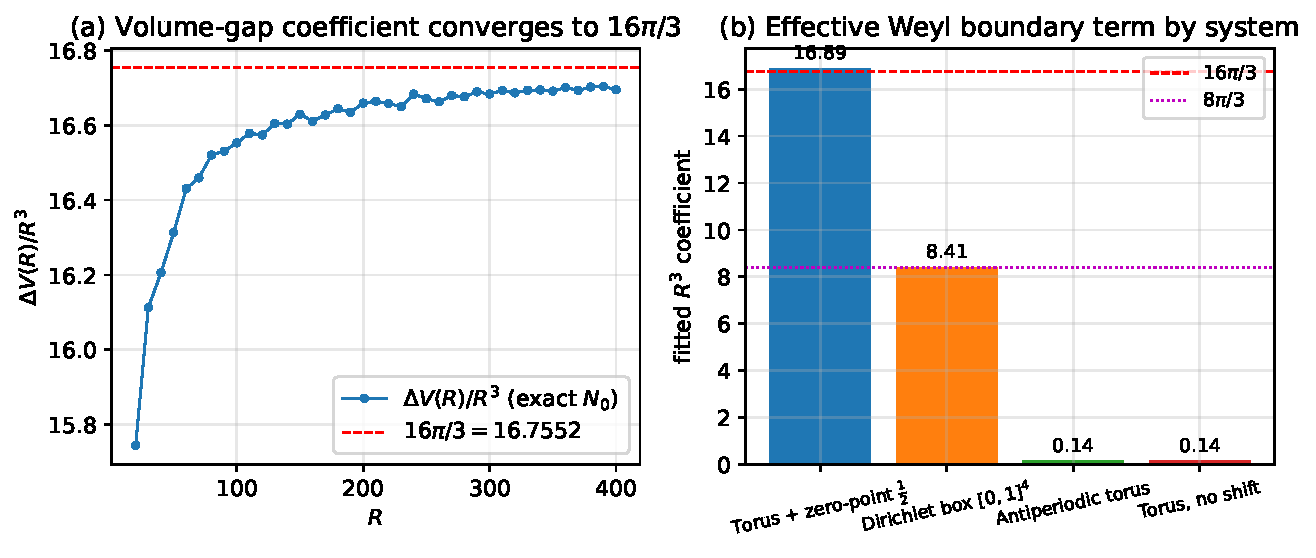
\includegraphics[keepaspectratio,alt={Figure 1. Convergence of the volume-gap coefficient and effective Weyl boundary terms}]{figure_paper5_1_weyl_gap_convergence.pdf}}

\textbf{Figure 1. Convergence of the volume-gap coefficient (left:
\(\Delta V/R^3\to16\pi/3\) from exact \(N_0\); right: fitted \(R^3\)
coefficients of the four boundary systems). The zero-point shift
generates an effective boundary exactly twice that of the Dirichlet unit
box.}

\subsubsection{4.2 Zero-point shift = effective
boundary}\label{zero-point-shift-effective-boundary}

Fitting the deficit \((\pi^2/2)R^4-N(R)\) by \(aR^3\)
(\(R=50\)--\(320\)) gives:

{\def\LTcaptype{none} % do not increment counter
\begin{longtable}[]{@{}lrl@{}}
\toprule\noalign{}
System & \(a\) (numerical) & Theoretical value \\
\midrule\noalign{}
\endhead
\bottomrule\noalign{}
\endlastfoot
Torus, real + zero point & 16.798 & \(16\pi/3=16.755\) \\
Antiperiodic & 0.042 & \(0\) (no \(R^3\) term) \\
Dirichlet box & 8.364 & \(8\pi/3=8.378\) \\
Torus, no zero point & 0.041 & \(0\) \\
\end{longtable}
}

A boundaryless torus intrinsically has no \(R^3\) term. The zero-point
half-shift generates a Weyl boundary term that is \textbf{exactly twice}
(\(16\pi/3=2\times8\pi/3\)) the Dirichlet boundary term of the unit box.
That is, the volume gap is the Weyl deficit expressing \textbf{that the
zero-point quantum acts as an effective boundary equivalent to
``Dirichlet walls facing both ways.''}

\begin{center}\rule{0.5\linewidth}{0.5pt}\end{center}

\subsection{5. Non-Overlap = Orthogonality, and Quantification of
Sparseness}\label{non-overlap-orthogonality-and-quantification-of-sparseness}

\subsubsection{5.1 Gram matrix}\label{gram-matrix}

Writing \(\Phi_k(x)=\prod_i\varphi_{k_i}(x_i)\) for the mode
corresponding to a cell \(k\) under the dictionary of §3.1, the
orthogonality of the 1-dimensional real Fourier basis and Fubini's
theorem give \(\langle\Phi_k,\Phi_{k'}\rangle_{L^2(T^4)}=\delta_{kk'}\).
Computing the Gram matrix of the 137 modes at \(R=3\) numerically,

\[
\max_{k,k'}\bigl|G_{kk'}-\delta_{kk'}\bigr| = 6.9\times10^{-16},
\]

which is the identity matrix to machine precision. \textbf{Cell
non-overlap and \(L^2\) orthogonality are the same sentence}: the
substance of fragments ``existing apart without touching'' is not
isolation by walls but orthogonality.

\subsubsection{5.2 Speckle statistics}\label{speckle-statistics}

For the intensity \(I=|\psi|^2\) of a phase-random superposition of the
137 orthogonal modes, the volume fraction with \(I>\kappa\bar I\) agrees
with the theoretical value \(e^{-\kappa}\) (\(\kappa=1\): measured
0.3691 versus theoretical 0.3679, etc.). The volume occupied by
constructive interference is \textbf{exponentially sparse} with respect
to the intensity threshold.

\begin{center}\rule{0.5\linewidth}{0.5pt}\end{center}

\subsection{6. The Coherence Condition and Completion of the Splitting
Theorem}\label{the-coherence-condition-and-completion-of-the-splitting-theorem}

\subsubsection{6.1 The odd rule}\label{the-odd-rule}

The representative value is
\(r_{\max}^2=\sum(\lvert k_i\rvert+\tfrac12)^2\in\{1,3,5,7,\ldots\}\):
\textbf{every odd number is realized, and no even number is realized}.
Realizability follows from Jacobi's four-square theorem
(\(16\sigma(m)>0\) for every odd \(m\)) {[}7{]}, and oddness from the
mod 8 arithmetic \((2k+1)^2\equiv1\pmod 8\). Therefore:

\begin{quote}
\textbf{Coherence condition}: A fragment can participate in the counting
at the parent level only if its representative value \(R'^2\) is an odd
integer.
\end{quote}

The Bohr-type coherence --- ``stable only when the wavelength fits an
integer number of times'' --- is thereby redefined not as a dynamical
stability condition but as \textbf{eligibility to participate in the
counting}.

\subsubsection{\texorpdfstring{6.2 The \(Z_2\) selection
rule}{6.2 The Z\_2 selection rule}}\label{the-z_2-selection-rule}

Since a sum of \(n\) odd numbers is congruent to \(n\pmod 2\), from
\(R^2=\sum_a R_a'^2\) we obtain:

\begin{quote}
\textbf{Selection rule}: the parity of the number of fragments in a
coherent splitting \(=\) the parity of \(R^2\).
\end{quote}

\subsubsection{6.3 Exception-free splitting
theorem}\label{exception-free-splitting-theorem}

For unrestricted integer partitions, there exist four exceptions
(\((14,1),\allowbreak(16,1),\allowbreak(20,1),\allowbreak(22,1)\)) to ``splitting decreases the
volume-gap indicator'' (non-monotonicity due to shell jumps of
\(g(s)\)). \textbf{All of them contain even parts and are entirely
eliminated by the coherence condition.} An exhaustive check of the 890
partitions into odd parts only with \(s\le25\) yields zero violations:

\begin{quote}
\textbf{Theorem}: Every coherent splitting of \(R^2\) (all parts odd,
two or more parts) strictly decreases the volume-gap indicator. The
all-ones partition is the unique global minimum.
\end{quote}

The coherence condition for interference waves and the stacking count
are not independent explanations; \textbf{the former is precisely the
condition that removes the exceptions from the latter's splitting
theorem}.

\pandocbounded{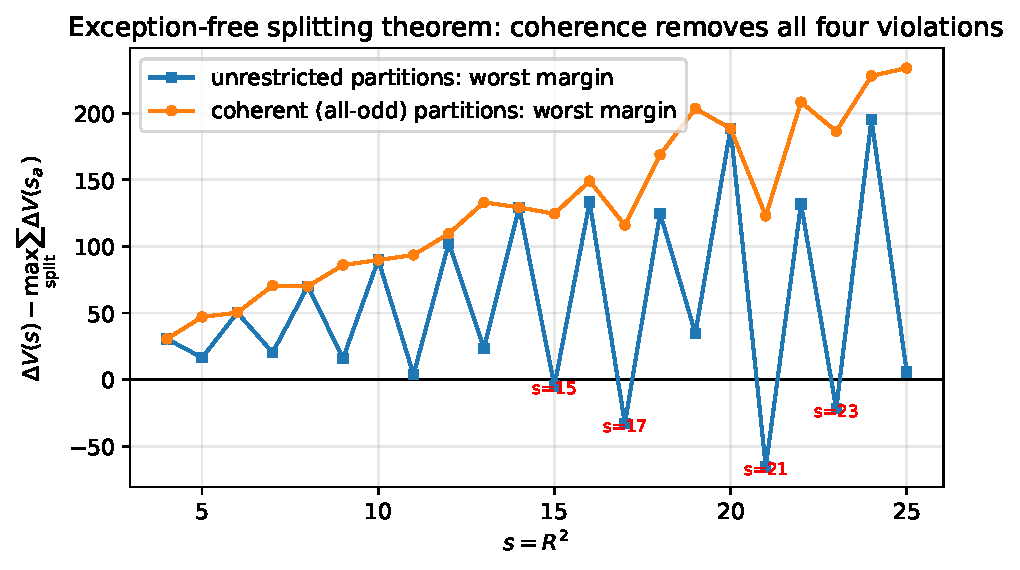
\includegraphics[keepaspectratio,alt={Figure 2. Exception-free splitting theorem under coherence}]{figure_paper5_3_splitting_theorem.pdf}}

\textbf{Figure 2. Exception-free splitting theorem: under unrestricted
partitions there exist four violations (\(s=15,17,21,23\)), all of which
are eliminated under coherent (all-odd) partitions (exhaustive for
\(s\le25\)).}

\subsubsection{6.4 Self-similar spectrum}\label{self-similar-spectrum}

The internal capacity \(N_0(\sqrt m)\) of a fragment at coherent label
\(m\) equals \(1,9,33,73,137,\ldots\) for \(m=1,3,5,7,9,\ldots\): the
representative-value spectrum and the capacity sequence are
\textbf{identical at every level of the hierarchy}. The self-similar
hierarchy of Paper 4 §9.3 is made rigorous at the level of label sets.

\pandocbounded{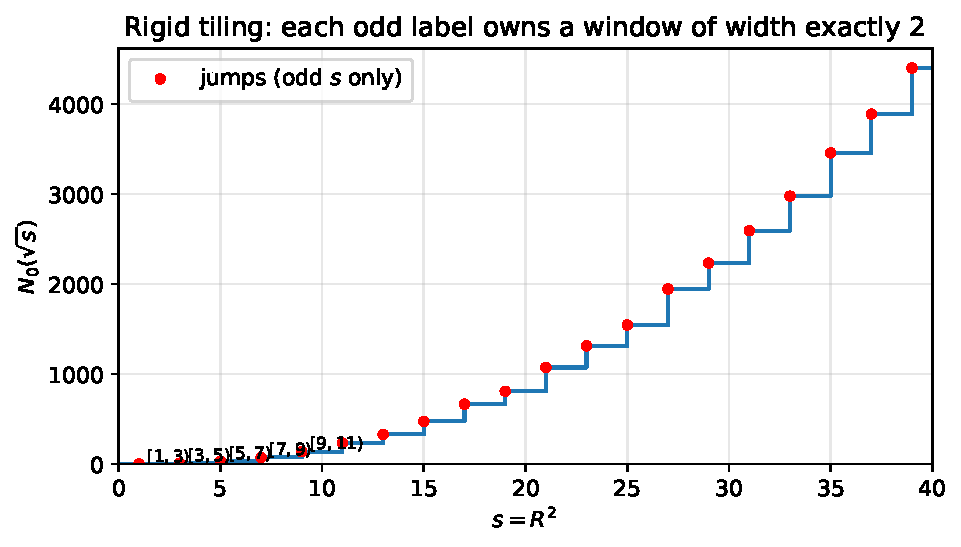
\includegraphics[keepaspectratio,alt={Figure 3. Rigid tiling of the energy axis by odd labels}]{figure_paper5_2_rigid_tiling.pdf}}

\textbf{Figure 3. Rigid tiling: jumps of \(N_0(\sqrt s)\) occur only at
odd \(s\), and each odd label owns a window of width exactly 2.}

\begin{center}\rule{0.5\linewidth}{0.5pt}\end{center}

\subsection{\texorpdfstring{7. The Classification Theorem for \(R^2\)
and the Resolution of Boundary
Criticality}{7. The Classification Theorem for R\^{}2 and the Resolution of Boundary Criticality}}\label{the-classification-theorem-for-r2-and-the-resolution-of-boundary-criticality}

\subsubsection{7.1 Classification theorem}\label{classification-theorem}

\begin{quote}
\textbf{Theorem (realizable spectrum)}: (i) The representative values of
single states take only odd integer values, and every odd integer is
realized. (ii) The composite values \(R^2=\sum_a s_a\) (\(s_a\) odd) of
composite states take only positive integer values and obey the \(Z_2\)
selection rule. (iii) Non-integer \(R^2\) is not realizable.
\end{quote}

As a corollary, among the points of the radius sweep of Paper 2, the
only state-theoretically realizable ones are those with integer
\(s=R^2\); the half-integer-\(R\) points are mathematical interpolation
values (a remark to be added to Paper 2 v0.3).

\subsubsection{7.2 Resolution of boundary
criticality}\label{resolution-of-boundary-criticality}

\(N_0(3)=137\) depends on the closed inequality \(\le\) (full inclusion
of the 64 cells of the boundary shell \(m=9\)), and the smoothing limit
of symmetric weight functions is \(73+64/2=105\). Once the
classification theorem is accepted, three independent arguments force
the closed inequality.

\begin{enumerate}
\def\labelenumi{\arabic{enumi}.}
\tightlist
\item
  \textbf{Absence of a continuous dial}: the smoothing limit presupposes
  that the cutoff radius can be moved continuously in a neighborhood of
  \(R=3\); but if the realizable \(R^2\) are quantized on the odd
  lattice, that limiting operation does not exist inside the system.
\item
  \textbf{Window structure of the tiling}: each odd label \(m\) owns the
  window \([m,m+2)\) on the \(s\) axis with width exactly 2, and the
  energy axis is tiled without gaps (jumps occur only at odd \(s\),
  confirmed for \(s\le40\)). Each window contains its left endpoint.
\item
  \textbf{Self-containment}: adopting the strict inequality \(<\), the
  state with label \(S\) would fail to fit within its own capacity,
  breaking the minimal requirement that ``a state owns its own shell.''
\end{enumerate}

\begin{quote}
\textbf{Reassessment}: ``137 or 105'' is not a question of arbitrariness
of normalization; it reduces to the difference between viewing \(R\) as
continuous (the diagnostic value 105 of the embedding) and viewing it as
an assemblable discrete value (the intrinsic value 137).
\end{quote}

\begin{center}\rule{0.5\linewidth}{0.5pt}\end{center}

\subsection{8. Closed Form of the Shell
Sequence}\label{closed-form-of-the-shell-sequence}

The shell count \(c(4m)\) (\(m\) odd) is given, with \(u_j(n)\) denoting
the number of ordered representations of \(n\) as a sum of \(j\)
positive odd squares, by

\[
c(4m) = 16\,\sigma(m) - 32\,u_3(4m-1) + 24\,u_2(4m-2) - 8\,u_1(4m-3) + [m{=}1]
\]

(expansion of the generating function \((2\theta-q)^4\); exact agreement
with direct counting for odd \(m\le199\)). Thus \(N_0(R)\) is positioned
not only within the geometry of numbers, but, via the divisor-sum
function, as an object of classical number theory.

\begin{center}\rule{0.5\linewidth}{0.5pt}\end{center}

\subsection{9. Scope of Claims of This
Paper}\label{scope-of-claims-of-this-paper}

What this paper claims: (1) the dictionary theorem (exact coincidence).
(2) The structural identification \(\delta_{\min}\) = zero-point
quantum. (3) The volume-gap leading term \(16\pi/3\) = the Weyl deficit
of the effective boundary (a conjecture strongly supported numerically;
a rigorous analytic proof is left as future work). (4) Non-overlap =
orthogonality (machine precision). (5) The coherence condition, the
\(Z_2\) selection rule, and the exception-free splitting theorem
(exhaustive check). (6) The classification theorem for \(R^2\) and the
intrinsic resolution of boundary criticality. (7) The closed form of the
shell sequence.

What this paper does not claim: (1) derivation of physical spacetime,
particles, or the vacuum. (2) Identification of \(\lambda,\nu\) with
physical quantities. (3) Identification of \(137\) with the
fine-structure constant. (4) A rigorous asymptotic expansion of the Weyl
term. (5) Explanation of cosmological numbers by speckle sparseness.

\begin{center}\rule{0.5\linewidth}{0.5pt}\end{center}

\subsection{10. Conclusion}\label{conclusion}

The lattice counting of Papers 1--4 is exactly identical to the counting
of real standing waves with zero-point shift. From this identification,
the identity of the minimal conjugate width (the zero-point quantum),
the identity of the volume gap (the Weyl deficit of the effective
boundary), the completion of the splitting theorem (elimination of
exceptions by the coherence condition), the classification theorem for
\(R^2\) (single states = odd integers), and the resolution of boundary
criticality (intrinsic forcing of the closed inequality) follow in a
chained manner, without additional assumptions.

\[
\begin{aligned}
&\text{zero point }\tfrac12\;\to\;\text{cells = real standing waves}\;\to\;\text{non-overlap = orthogonality}\\
&\quad\to\;\text{odd-rule coherence}\;\to\;\text{exception-free splitting}\;\to\;\text{quantization of }R^2
\end{aligned}
\]

This chain forms the mathematical foundation for the subsequent papers
(condensation and expansion, configuration statistics, stability).

\begin{center}\rule{0.5\linewidth}{0.5pt}\end{center}

\subsection{Appendix: Key Points of the Reproduction
Procedure}\label{appendix-key-points-of-the-reproduction-procedure}

All numerical verifications are reproducible with integer arithmetic or
double-precision arithmetic. The mode-count comparison uses convolution
of per-axis (value, weight) lists; the Weyl fit uses least squares over
\(R=50\)--\(320\); the Gram matrix uses a discrete orthogonal grid (8
points per axis); the coherent-partition check uses exhaustive
enumeration of the 890 odd partitions with \(s\le25\). The scripts and
research notes are provided in the public repository
(https://github.com/WurabeSeiji/ai-chat-logs-open , in the ``Dual
Geometry of Wavelength Space and Frequency Space'' folder).

\begin{center}\rule{0.5\linewidth}{0.5pt}\end{center}

\subsection{References}\label{references}

{[}1{]} Noriaki Kihara, ``Paper 1: Dual Geometry of Wavelength Space and
Frequency Space,'' v0.3, 2026. Concept DOI: 10.5281/zenodo.20588036.

{[}2{]} Noriaki Kihara, ``Paper 2: Radius Sweep of Fully-Inscribed
Unit-Cell Counts on a 4-Dimensional Lattice,'' v0.2, 2026. Concept DOI:
10.5281/zenodo.20588038.

{[}3{]} Noriaki Kihara, ``Paper 3: Closed Four-Dimensional Structure and
Lattice-Counting Supplement,'' v0.3, 2026. Concept DOI:
10.5281/zenodo.20589261.

{[}4{]} Noriaki Kihara, ``Paper 4: Splitting of Reciprocal Dual Cells
and Hierarchical State Structure,'' v1.0, 2026. Concept DOI:
10.5281/zenodo.20638962.

{[}5{]} H. Weyl, ``Über die asymptotische Verteilung der Eigenwerte,''
Nachr. Königl. Ges. Wiss. Göttingen (1911), 110--117.

{[}6{]} M. Kac, ``Can one hear the shape of a drum?,'' American
Mathematical Monthly 73(4) (1966), 1--23.

{[}7{]} G. H. Hardy and E. M. Wright, \emph{An Introduction to the
Theory of Numbers}, 6th ed., Oxford University Press, 2008.

{[}8{]} J. H. Conway and N. J. A. Sloane, \emph{Sphere Packings,
Lattices and Groups}, 3rd ed., Springer, 1999.

{[}9{]} R. Courant and D. Hilbert, \emph{Methods of Mathematical
Physics}, Vol. I, Interscience, 1953.

\begin{center}\rule{0.5\linewidth}{0.5pt}\end{center}

\subsection{License}\label{license}

This paper is published under CC BY 4.0.\\
Reuse, adaptation, translation, and citation are permitted, provided
that the author name, version, publication date, and source are clearly
indicated.

\end{document}
